\documentclass[a4paper,11pt]{jsarticle}


% 数式
\usepackage{amsmath,amsfonts}
\usepackage{bm}
\usepackage{physics}
% 画像
\usepackage[dvipdfmx]{graphicx}
% ローマ数字
\usepackage{otf}
% 単位
\usepackage{siunitx}
% 表
\usepackage{multirow}
% 化学反応
\usepackage[version=4]{mhchem}

\begin{document}

\title{理論演習 ランダム触媒反応ネットワーク}
\author{齋藤駿一}
\date{\today 編集}
\maketitle

\section{概要}
古澤先生(2003)のモデルを参考にして,ランダムな触媒反応ネットワークを用いた細胞モデルを作成した.
本モデルでは濃度ベースの記述を採用し,体積増大はある1種類の分子(膜分子)からの化学反応によってのみ起こるとした.
ここではこのモデルに基づき,定常的に成長する反応ネットワークが出現する確率を調べた.

\section{モデル}
\subsection{設定}
まず,細胞内に化学種$i=0,\cdots, N-1$が存在すると仮定し,その濃度を$x_i$とおく.
加えて,一般性を失わずに,$i=0$を膜分子,$i=1,\cdots, fN$を細胞を透過できる化学種(栄養)と仮定する.
ここで,$f$は化学種全体のうち膜を透過できるものの割合を示している.
また,細胞の体積を$V$とおく.

次に,以下の方法で確率的に触媒反応$\ce{$i$ + $k$ -> $j$ + $k$}$を構築する.
\begin{enumerate}
  \item 任意の異なる2種の組$(i,j)$に対し,ある確率$p$で反応経路$\ce{$i$ -> $j$}$を繋ぐ.
  \item 各反応に対し,それを触媒する成分$k$を($i,j$自身を含む全成分から)ランダムに選ぶ.
\end{enumerate}
こうしてできた反応$\ce{$i$ + $k$ -> $j$ + $k$}$により,単位時間で成分$i$は$\epsilon x_i x_k$減少し,成分$k$はこれと同じだけ増加すると仮定する.
ここで,反応速度$\epsilon$は全反応に共通であるとする.

また,細胞を透過できる化学種$i$については,膜透過による濃度変化も考える.
具体的には,それらの成分の細胞外での濃度を$\bar{x}_i$とし,単位時間あたりに濃度勾配に比例した流入$D(\bar{x}_i - x_i)$があると考える.
ここでは$D$を拡散係数と呼び,これは全成分について共通であるとする.

最後に,膜分子$i=0$は$\epsilon_g x_0$のレートで減少し,体積は
\begin{equation}
  \frac{dV}{dt} = \mu V = g \epsilon_g x_0 V
\end{equation}
のように増加すると仮定する.
これに伴い,全成分が成長速度$\mu=g \epsilon_g x_0$で希釈されると考える.

まとめると,膜透過しない成分の濃度は触媒反応と希釈によって変化する.
膜透過する成分の場合はここに拡散流入が加わり,膜分子の場合は膜形成が加わる.

\subsection{「分裂」操作}
こうしてできたモデルを適当な初期値(ここでは全成分一様濃度,$V=1$)から時間発展させる.
このとき$V$がはじめて2を超えたところで,濃度を一定に保って体積を半分にするという操作(「分裂」と呼ぶ)を挟む.
これを数回繰り返して,(細胞が成長する場合に)濃度が定常になることを確認する.

この「分裂」操作により,細胞が定常的に成長できるかを確認できる,
もし数回の分裂の後に全成分が定常濃度に至るなら,その細胞は定常的に成長するといえる.
一方で,定常濃度に至る前に成長が止まる\footnote{プログラムの都合で,体積が2倍になる制限時間を設けている.もし制限時間になっても体積が2倍にならなければ,この細胞は「成長に失敗した」と判断する.}なら,細胞は定常的に成長しないといえる.

\section{計算内容とその結果}
ここでは,成分の種類は$N=10$とし,$g,\epsilon_g,\epsilon,D$および環境の栄養濃度$n$をすべて1として計算した.
また,「分裂」の制限時間は10とした.

\subsection{何回か計算}
$p=0.8, f=0.1$\footnote{$f=0.1=1/N$は栄養分子が1つという場合に相当する.}で計算を行うと,基本的に定常的な成長が確認できた.
一方,$p=0.3$に変更すると,定常的な成長をしない場合も見られた.

\begin{figure}[htbp]
  \centering
  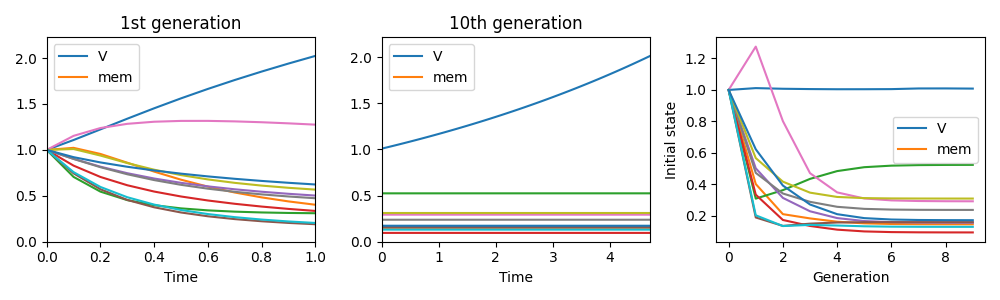
\includegraphics[width=\columnwidth]{rand_05_01_1.png}
  \caption{$p=0.8,f=0.1$の場合.左の図は最初の世代の挙動,中央の図は10世代目の挙動を表す.右の図は初期状態とその後の「分裂」直後の状態の推移を表す.}
  \label{fig:rand_08_01}
\end{figure}

\begin{figure}[htbp]
  \centering
  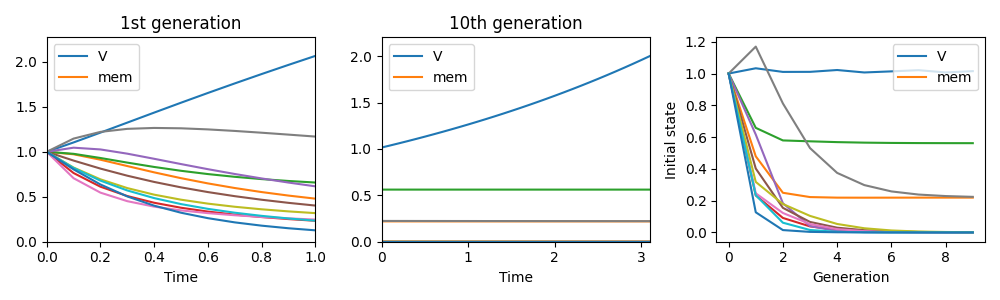
\includegraphics[width=\columnwidth]{rand_03_01_1.png}
  \caption{$p=0.3,f=0.1$の場合(1).}
  \label{fig:rand_03_01_1}
\end{figure}
\begin{figure}[htbp]
  \centering
  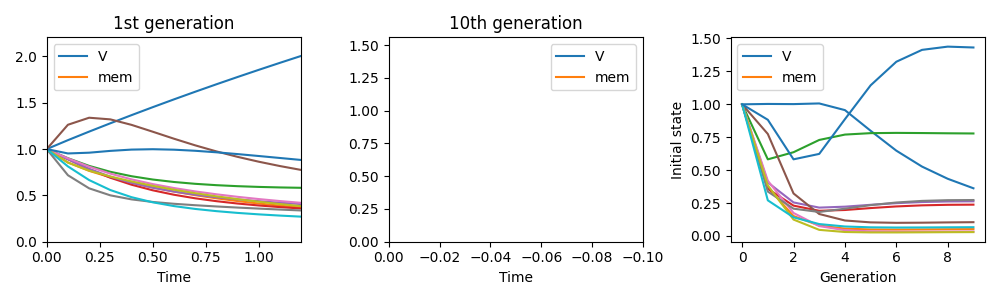
\includegraphics[width=\columnwidth]{rand_03_01_2.png}
  \caption{$p=0.3,f=0.1$の場合(2).4世代目で「分裂」が間に合わず,成長が止まった.(これ以降の計算は無意味なので無視して良い.)}
  \label{fig:rand_03_01_2}
\end{figure}

\subsection{Connection rate $p$と生存率の関係}
上の結果から,反応のpathを繋げる確率$p$を変えると,細胞が定常的に成長する確率が変わることが分かる.
そこで,次にこの関係を詳しく調べた.

まず,$p$を0から1まで0.1刻みで変化させ,それぞれの$p$に対して30通りずつ反応ネットワークを組んで,一様濃度から時間発展させた.
ここで,簡単のため栄養分子を1分子のみとした($f=1/N$).
そして,この30通りのうち,10世代目まで定常的に成長した(10回目の「分裂」直後の体積が1以上となる)ネットワークの割合を「生存率」と呼ぶことにし,$p$に応じて生存率がどう変わるかを調べた.

その結果,図\ref{fig:ps30_2}のような緩やかな立ち上がりが見られた.
ここで,プロット点だけでは意味が分かりづらいので,補助的に曲線を描いた.
この曲線は,栄養分子から反応のpath(矢印)を辿っていって膜分子に到達できる理論的な確率を表す(導出は付録に載せた).
この確率が生存率よりも高いことは直感に合う.
また,この2つの確率の差は,自己触媒サイクルを作ることの難易度と捉えられる.


\begin{figure}[htbp]
  \centering
  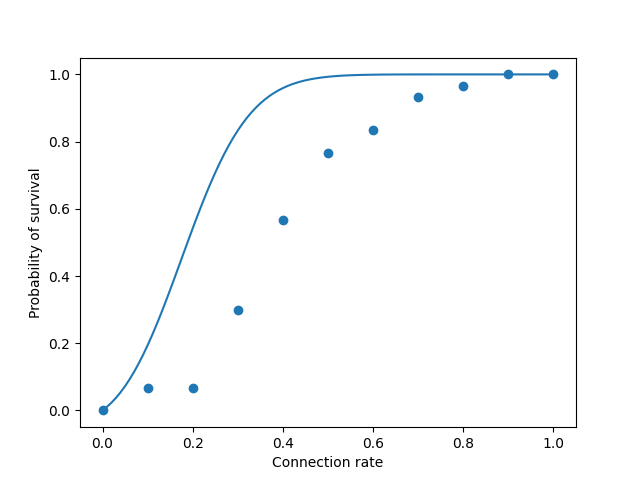
\includegraphics[width=10cm]{ps30_2.png}
  \caption{$f=0.1$におけるConnection rate $p$と生存率の関係(点)および栄養分子から反応ネットワークの矢印を辿って膜分子に到達できる理論的な確率(曲線).}
  \label{fig:ps30_2}
\end{figure}

\begin{figure}[htbp]
  \centering
  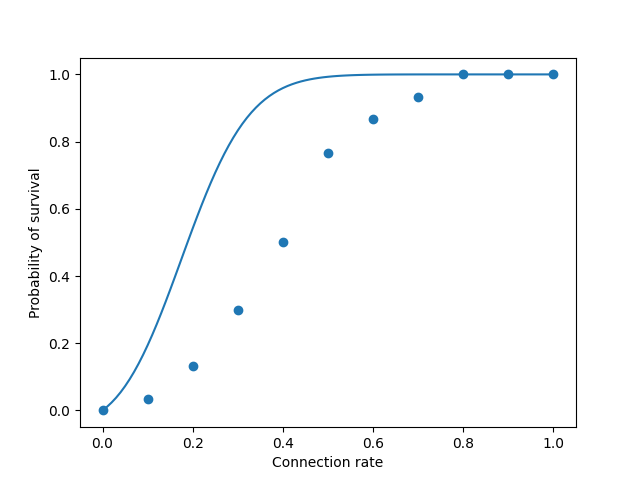
\includegraphics[width=10cm]{ps30_3.png}
  \caption{図\ref{fig:ps30_2}と同じ計算をもう一度行い,再現性を確かめた.}
  \label{fig:ps30_3}
\end{figure}

\subsection{栄養成分の割合$f$と生存率の関係}
次に,$p=0.3$と固定し,栄養成分の割合$f$を変えていって生存率を計算した.
こちらはランダム性によるゆらぎが大きかったので,60通りの反応ネットワークを作って生存率を求めた.
その結果,図\ref{fig:psf60_1}および図\ref{fig:psf60_2}が得られた.
こちらも緩やかな立ち上がりが見られたが,栄養成分の割合を増やすだけでは生存率は頭打ちになることが分かった.

\begin{figure}[htbp]
  \centering
  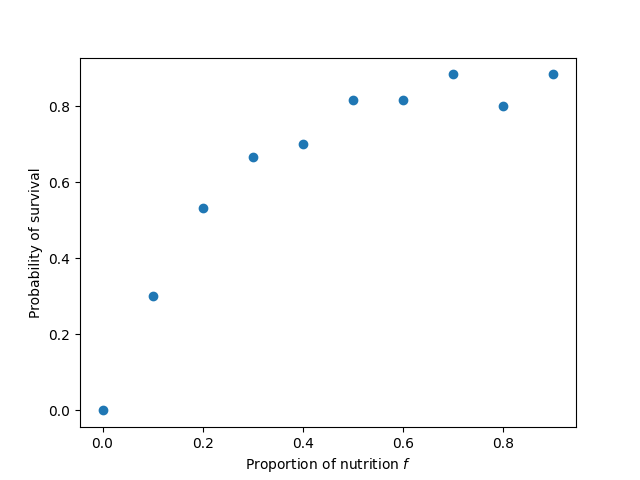
\includegraphics[width=10cm]{psf60_1.png}
  \caption{$p=0.3$における栄養成分の割合$f$と生存率の関係.}
  \label{fig:psf60_1}
\end{figure}

\begin{figure}[htbp]
  \centering
  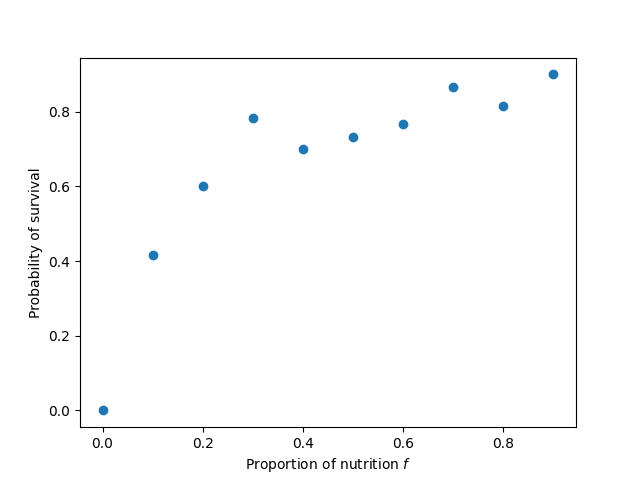
\includegraphics[width=10cm]{psf60_2.png}
  \caption{図\ref{fig:psf60_1}と同じ計算をもう一度行い,再現性を確かめた.}
  \label{fig:psf60_2}
\end{figure}

この「頭打ち」は$p=0.9$としても見られた(図\ref{fig:psf60_3_09}).

\begin{figure}[htbp]
  \centering
  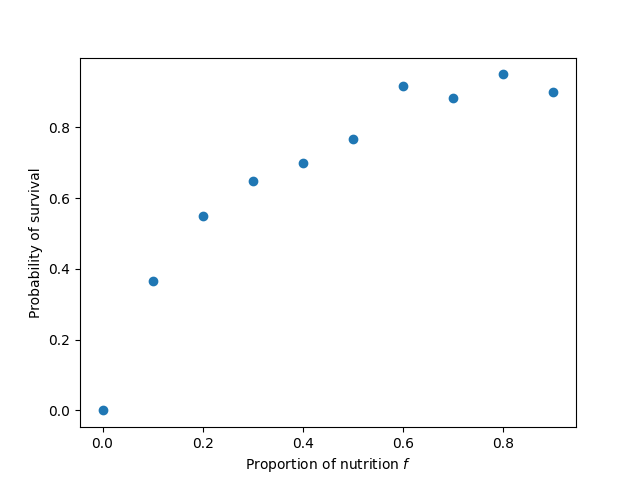
\includegraphics[width=10cm]{psf60_3_09.png}
  \caption{$p=0.9$における栄養成分の割合$f$と生存率の関係.}
  \label{fig:psf60_3_09}
\end{figure}

\section{付録:図の曲線の導出}
成分が$N$種類のとき,栄養分子から膜分子まで反応のpathを辿って到達できる確率を$P_{N}$とおく.
ここでは,この確率$P_{N}$を帰納的に導出する.

まず,$N=2$のとき,栄養分子と膜分子しか存在しないので,その間にpathができる確率は$p$である.
\begin{equation}
  P_2 = p
\end{equation}

次に,$P_{N+1}$を$P_{N}$で表す.
成分が$N$種あるとき,それを栄養分子と膜分子とその残り$N-2$種に分けることができる.
このとき,栄養分子から膜分子へ(直接または$N-2$種のどれかを経由して)反応を辿れる確率が$P_N$である.
一方,成分が$N+1$種のときは,栄養分子と膜分子以外の成分を,$N-2$種(A)と残り1種(B)に分けることができる.
この状況で確率$P_{N+1}$を考える.
まず,直接またはAのどれかを経由して栄養分子から膜分子に辿り着く確率は$P_{N}$である.
次にそうでない場合(確率$1-P_{N}$)を考えると,このときは栄養分子から直接またはAのどれかを経由してBにたどり着き,かつBから膜分子に矢印が伸びていれば良い.
したがって,その確率は$(1-P_{N})\times P_{N}\times p$である.
以上より,
\begin{equation}
  P_{N+1} = P_{N} + p(1-P_{N})P_{N}
\end{equation}
が導かれる.

図の曲線はこの漸化式をもとに$P_{10}$を数値計算してプロットした.

\end{document}